% !TEX root = main-crime.tex
\section{Experiments}
\label{ch2-sec:experiment}


\subsection{Settings}


We adopt leave-one-out evaluation to estimate the crime rate of one geographic region given all the information of all the other regions. When we construct the spatial/social lag variable for the training data, the effect of testing region is completely removed. For example, if region $y_t$ is the testing region, the remaining $\{y_i\} \backslash y_t$ become the training set. For any $y_j$ in the training set, its geographical influence feature and taxi flow feature are constructed from $\{y_i\} \backslash \{y_t, y_j\}$.


In the evaluation, we estimate the crime rate for testing community areas. The accuracy of estimation is evaluated by mean absolute error (MAE) and mean relative error (MRE).

\begin{align}
MAE & = \frac{\sum_i^n |y_i - \hat{y_i}| }{n} \\
MRE & = \frac{\sum_i^n |y_i - \hat{y_i}|} {\sum_i^n y_i }
\end{align}







\subsection{Performance Study}


We evaluate the estimation accuracy under various feature combinations. The leave-one-out evaluation results are shown in Table~\ref{tb:perf}.  We run both the linear regression and the negative binomial regression on five consecutive years, 2010 -- 2014. Both MAE and MRE are shown in the table. We have four types of features: demographics, POI, geographical influence and taxi flow. We test the various settings of feature combinations.





\begin{table*}[htb]
\centering
\caption{Performance evaluation. Various feature combinations are shown in each column. The linear regression model and negative binomial results are compared by year group.}
\vspace{2mm}
\label{tb:perf}

\resizebox{\columnwidth}{!}{%


\begin{tabular}{|c|c|c|c|c|c|c|c|c|c|c|}
\hline
\multicolumn{3}{|c|}{} & \multicolumn{8}{|c|}{Settings} \\ \hline
\multicolumn{3}{|c|}{Column ID} & 1 & 2 & 3 & 4 & 5 & 6 & 7 & 8 \\ \hline
\multicolumn{2}{|c|}{\multirow{4}{*}{Features$^1$}}	& \textbf{D}emo & \checkmark & \checkmark&\checkmark & \checkmark & \checkmark& \checkmark& \checkmark& \checkmark \\ \cline{3-11}
\multicolumn{2}{|c|}{}	& \textbf{G}eo & & & & & \checkmark & \checkmark& \checkmark& \checkmark \\ \cline{3-11}
\multicolumn{2}{|c|}{}	& \textbf{P}OI & & \checkmark & & \checkmark & &\checkmark & & \checkmark \\ \cline{3-11}
\multicolumn{2}{|c|}{}	& \textbf{T}axi & & & \checkmark& \checkmark & & & \checkmark& \checkmark \\ \hline
Year & Model$^2$ & Error & \multicolumn{8}{|c|}{} \\ \hline
	\cellcolor{white}&  \cellcolor{white} & MAE & 394.41 & 416.98 & 408.09 &  406.93  &394.78 &432.45 & 402.25& 416.41\\ \cline{3-11}
	&	\multirow{-2}{*}{LR}& MRE & 0.294& 0.311 & 0.304 & 0.304 & 0.295 &0.323 & 0.300& 0.310\\ \hhline{|~|*{10}{-|}}
	\rowcolor{Gray}
	\cellcolor{white}	& \cellcolor{white} & MAE & 391.53&   333.14 & 395.64 & 323.47 & 389.55&350.06 & 387.43& \textbf{320.75}\\ \hhline{|~|~|*{9}{-|}}
	\rowcolor{Gray}
	\cellcolor{white}\multirow{-4}{*}{2010}	&\cellcolor{white}\multirow{-2}{*}{NB}	& MRE & 0.292& 0.249 & 0.295 & 0.241 & 0.290& 0.261& 0.289& \textbf{0.239} \\ \hline
	


	\cellcolor{white}	& \cellcolor{white} & MAE & 380.22&   409.30 & 396.97 &  401.11 & 379.61& 422.94&389.39 & 408.91\\ \cline{3-11}
	&	\multirow{-2}{*}{LR}& MRE &0.295  &  0.318  &  0.309 &  0.312 & 0.295 &0.328 & 0.302 & 0.320   \\ \hhline{|~|*{10}{-|}}
	\rowcolor{Gray}
	\cellcolor{white}& \cellcolor{white} & MAE &381.11 & 332.62 & 388.81  & 328.94 & 378.84& 345.24& 381.33& \textbf{335.97} \\ \hhline{|~|~|*{9}{-|}}
	\rowcolor{Gray}
	\cellcolor{white}\multirow{-4}{*}{2011}	&	\cellcolor{white}\multirow{-2}{*}{NB}& MRE&0.296 & 0.259 & 0.302  & 0.256 & 0.294 & 0.268  & 0.296  & \textbf{0.253}  \\ \hline
	


	\cellcolor{white}& \cellcolor{white} & MAE &378.91 & 412.95 & 401.54  & 412.20& 376.53 & 423.88 & 399.25 & 419.93\\ \cline{3-11}
	&	\multirow{-2}{*}{LR}& MRE& 0.306 & 0.334 & 0.325 & 0.333&  0.304 & 0.343 & 0.322 & 0.339 \\ \hhline{|~|*{10}{-|}}
	\rowcolor{Gray}
	\cellcolor{white}& \cellcolor{white} & MAE & 386.31 & 337.24 & 389.58  & 331.41 & 384.23 & 352.22 & 381.67 & \textbf{345.49} \\ \hhline{|~|~|*{9}{-|}}
	\rowcolor{Gray}
	\cellcolor{white}\multirow{-4}{*}{2012}&\cellcolor{white}\multirow{-2}{*}{NB}	& MRE& 0.312 & 0.273 & 0.315  & 0.268 & 0.310 & 0.284 & 0.308 & \textbf{0.279} \\ \hline
	

	\cellcolor{white}& \cellcolor{white} & MAE & 367.89 & 420.81 & 390.75  & 402.75 & 369.24 & 433.48 &388.92 & 412.31\\  \cline{3-11}
	&	\multirow{-2}{*}{LR}& MRE& 0.324 &  0.370 & 0.344  & 0.354  & 0.325 & 0.381 & 0.342& 0.362\\ \hhline{|~|*{10}{-|}}
	\rowcolor{Gray}
	\cellcolor{white}& \cellcolor{white}& MAE & 376.08&  333.92 & 373.08 & 312.63 & 377.57 & 350.33 & 368.49 & \textbf{319.86}\\ \hhline{|~|~|*{9}{-|}}
	\rowcolor{Gray}
	\cellcolor{white}\multirow{-4}{*}{2013}	&	\cellcolor{white}\multirow{-2}{*}{NB} & MRE& 0.331 &   0.294 & 0.328  & 0.275 & 0.332 & 0.308 & 0.324& \textbf{0.281}\\ \hline

	\cellcolor{white}& \cellcolor{white} & MAE & 331.28 & 375.53 & 349.00  & 350.31 & 329.93& 386.90& 345.79& 361.28\\  \cline{3-11}
	&	\multirow{-2}{*}{LR} & MRE& 0.326 & 0.369 & 0.343  & 0.345 & 0.324& 0.380& 0.340& 0.355\\ \hhline{|~|*{10}{-|}} 
	\rowcolor{Gray}
	\cellcolor{white}&\cellcolor{white}  & MAE & 340.73 & 293.52  & 339.17  & 274.45 & 336.09& 308.18& 326.07& \textbf{273.27}\\ \hhline{|~|~|*{9}{-|}}
	\rowcolor{Gray}
	\cellcolor{white}\multirow{-4}{*}{2014}	&	\cellcolor{white}\multirow{-2}{*}{NB}& MRE& 0.335&  0.289 & 0.334 & 0.270 &  0.331 & 0.303& 0.321 & \textbf{0.269}\\ \hline
\end{tabular}
}

\footnotesize{$^1$ D -- demographic features, G -- geographical influence, P -- POI features, T -- taxi flow feature.\\}
\footnotesize{$^2$ LR -- Linear Regression, NB -- Negative Binomial Regression.}
\end{table*}



%\medskip
%\noindent \textbf{Negative binomial regression vs. linear regression.} 
\subsubsection{Negative Binomial Regression vs. Linear Regression}
In Table~\ref{tb:perf},  we can see that in different years and under most settings, the negative binomial regression significantly outperforms the linear regression (with only a few exceptions when using only demographic feature). When using all the features, NB is significantly better than LR with at least $6\%$ improvement in relative error.
One reason is that negative binomial regression is a count prediction model, which guarantees the prediction variable is non-negative . Another reason is that it is difficult to get very precise estimates of crime rate, and the negative binomial regression allows a large variance in the estimated crime rate. Therefore negative binomial is more appropriate for crime rate estimation than linear regression.

In the following discussions, we only refer to the performance of the negative binomial regression.




%\medskip
%\noindent \textbf{POI feature.} 
\subsubsection{POI Feature} Adding POI features always improves the accuracy (see NB for column 2 vs. column1, column 6 vs. column 5, column 8 vs. column 7). The POI distribution reflects the functionality of a region. The most correlated POI major category is ``professional'', under which there are a lot of venues like transportation center and conventional center. These are locations with more dynamic movements of people. Such location information is not reflected in any of other features. POI thus provides  unique information and it shows that using big data can benefit us in advancing the study of traditional crime inference problems. 

Another issue that is worth discussing is whether POI is a surrogate of population features from demographics. That is, a region with POIs is a region with a higher population. However, as we see from Table~\ref{tb:perf}, adding POI in addition to demographics always outperforms the features without POI. This is because population from demographics reflects the number of residents in that region, but POI reflects dynamics of population (e.g., people go to venues for food, entertainment, or travel). Therefore, the dynamic population in POI further complements the residential population in demographics.



\vspace{2mm}
\subsubsection{Taxi Flow} 
The taxi flow is shown to improve the inference accuracy (see NB for column 3 vs. column 1, column 7 vs. column 5, column 8 vs. column 6). 
This validates our hypothesis that crimes do not only correlate with nearby regions but also correlate through hyperlinks on the space (i.e., the taxi flow). 

Comparing column 7 (D+G+T) with column 5 (D+G), we find that the improvement by taxi flow is not obvious. However, comparing column 8 (D+G+P+T) with column 6 (D+G+P), we observe a much significant accuracy boost. The reason could be that the taxi flow further complements the POI data. When POI information is missing from the predictor, the city dynamics captured by taxi flow are weakened as well.


\vspace{4mm}
\subsection{Feature Construction}


There are different ways to use the POI and taxi datasets. In this section, we share our insights into the more effective ways in constructing the features. 

\begin{figure}[t]
\centering
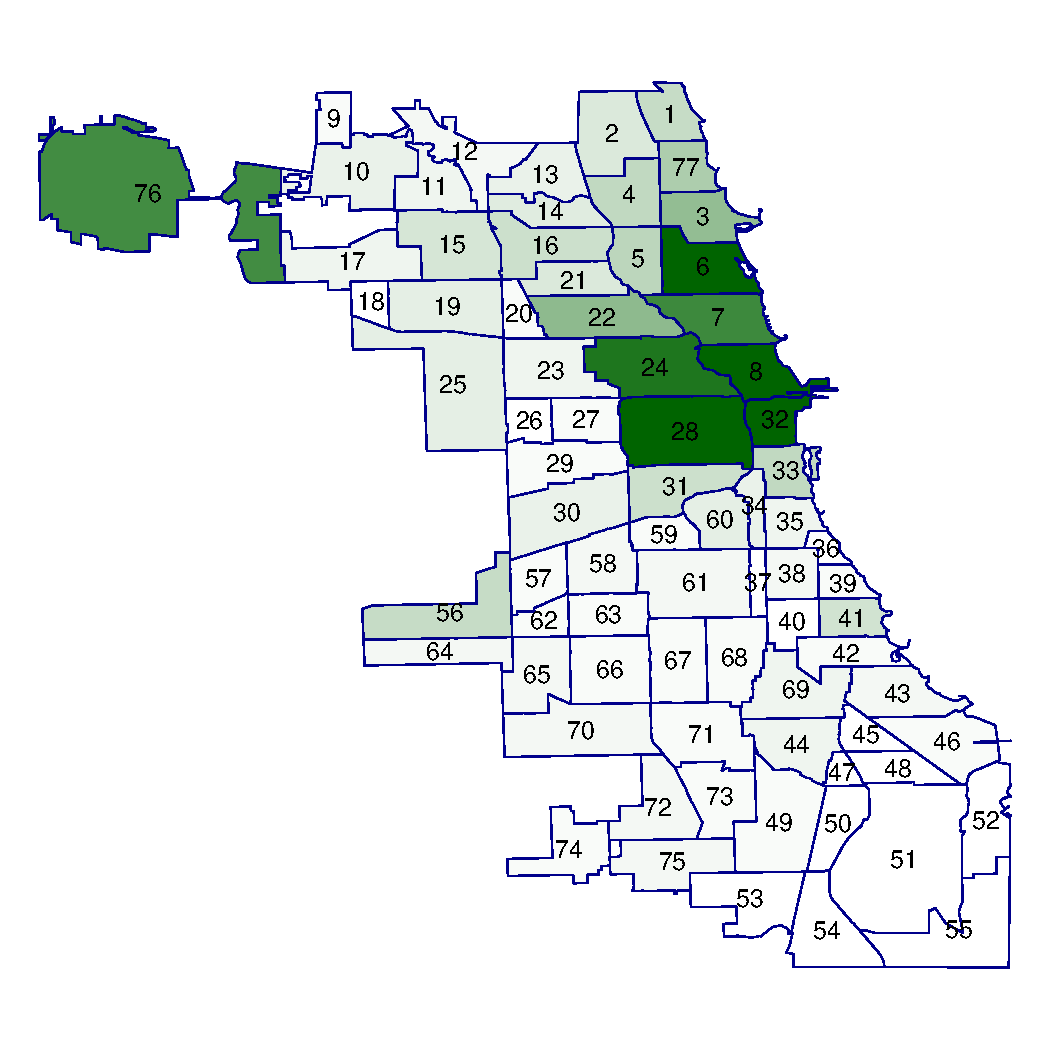
\includegraphics[width=0.7\textwidth]{fig/poi-cnt3.pdf}
\caption{Absolute POI count distribution. In our crawled POI dataset, most community areas have less than 100 venues. Meanwhile, the downtown area there are over $10,000$ venues for one community area, e.g. \#8, \#32.}
\label{fig:poi-dist}
\end{figure}

\vfill\eject
\subsubsection{POI Normalization}
The straightforward definition of POI distribution is calculated by normalizing the POI count in each category by the total POI counts. However, the POIs in Chicago are not evenly distributed. As shown in Figure~\ref{fig:poi-dist}, most POIs are in the downtown area and some areas only have a few POIs. If normalized by the total number of POIs in a neighborhood, two neighborhoods may show similar distributions but they are quite different. For example, a downtown neighborhood and a distant neighborhood may both have a high ratio of the food category but the downtown neighborhood has many more POIs in total and is more dynamic in population constitution. Therefore, using the raw count instead of normalized distribution is more effective. This is also demonstrated in estimation accuracy as shown in Table~\ref{tb:poi-norm}. 

\begin{table}[h]
\centering
\caption{Using POI count instead of POI percentage improve the estimation accuracy. Estimation for crime in 2014 with all other features.}
\vspace{2mm}
\label{tb:poi-norm}
\begin{tabular}{|c|c|c|}
\hline
\multirow{2}{*}{Scheme} & \multicolumn{2}{|c|}{NB} \\ \cline{2-3}
	& MAE & MRE \\ \hline
POI count & 273.27& 0.269  \\ \hline
POI percentage &283.16  & 0.278\\ \hline
\end{tabular}
\end{table}




%\medskip
%\noindent \textbf{Taxi Flow normalization.} 
\subsubsection{Taxi Flow Normalization}
The taxi flow represents the interactions among community areas. There are several different approaches to incorporate the taxi flow into the model.  First, we can use the raw taxi count as a weight on crime from other neighborhoods. One issue with the raw count is the concentration of taxi trips distribution in the downtown area. Consider the following example. In the downtown area, the average taxi flow count is \num{1000} between any pair of community areas, while the average of suburbs is $100$. When we propagate crime by raw taxi count, the same amount of crime in downtown is propagated with a  $10$ times higher coefficient than that of suburb. 


To address this issue, we can normalize the taxi flow, and there are two different approaches to normalize. 1) We can normalize the taxi flow by the total incoming traffic of the destination community area, and the semantics of this normalization is splitting the crime in the destination to all its neighbors. 2) Alternatively, we can normalize the taxi flow by the outgoing total trips in the source community area. This normalization assumes the crime in each source community is spread out by the flow.  The two normalization methods are shown in Figure~\ref{fig:taxiflow-norm}.


\begin{figure}[h]
\centering
\begin{tikzpicture}
\node[right]  at (0,0) {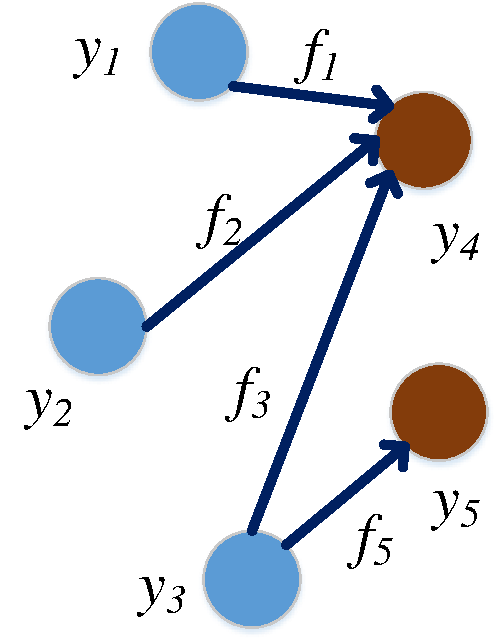
\includegraphics[width=0.12\textwidth]{fig/taxiflow-normalization.pdf}};
\node[align=left, above right] at (2.3, 0.3) {Normalization by source: \\ $F^t_4 = \frac{f_1}{f_1} y_1 + \frac{f_2}{f_2} y_2 + \frac{f_3}{f_3+f_5} y_3$};
\node[align=left, below right] at (2.3, -0.3) {Normalization by destination:  \\ $F^t_4 = \frac{f_1}{f_1+f_2+f_3} y_1 + \frac{f_2}{f_1+f_2+f_3} y_2 + \frac{f_3}{f_1+f_2+f_3} y_3$};
\end{tikzpicture}
\caption{Two different normalization schemes.}
\label{fig:taxiflow-norm}
\end{figure}



\begin{table}[h]
\centering
\caption{Various approaches to construct taxi flow feature. Estimation for crime in 2013 with all other features.}
\vspace{2mm}
\label{tb:tf-design}
\begin{tabular}{|l|c|c|}
\hline
\multirow{2}{*}{Settings} & \multicolumn{2}{|c|}{NB} \\ \cline{2-3}
	& MAE & MRE \\ \hline
Taxi flow count & 368.71 & 0.324 \\ \hline
Taxi flow normalized by source & 349.38 & 0.307 \\ \hline
Taxi flow normalized by destination & 319.86& 0.281\\ \hline
\end{tabular}
\end{table}


In Table~\ref{tb:tf-design} we compare the different approaches to handle the taxi flow. Using raw taxi flow count is clearly not a good option, due to the unbalanced data distribution. We also observe that normalizing taxi flow by destination is better than normalization by source. The reason could be explained by the example given in Figure~\ref{fig:taxiflow-norm}. Suppose the focal region is a transportation hub, which has a lot of isolated regions connected to it. If we normalize the crime by source region, then the taxi flow feature of focal region is overestimated, since the coefficients of its neighbors do not sum to one. 




\subsection{Feature Importance}

In this subsection, we study the importance of features through significance tests and coefficient changes over the years.


\subsubsection{Significance Test} 
From previous results, we see that combining POI features and taxi flow will help improve the estimation accuracy. Now we try to measure the significance of this accuracy boost by permutation tests. If a feature correlates with crime, when we randomly permute the values of this feature among neighborhoods, we will expect a higher error in crime estimation. So in each round of permutation, we can get an error in estimation. We compare the error with the original feature to the error distribution obtained from permutations. We conduct 1,000 rounds of permutations to approximately estimate the error distribution. The position of the original error in this distribution indicates the significance of this feature. For example, if the original error is smaller than 99\% of the errors from the permutations, the p-value is 0.99. 

\nop{
The permutation test procedure is described as follows. Each feature is randomly permuted for $1,000$ times. After each permutation, the leave one out evaluation is applied to get the accuracy measure (MAE, MRE). The $1,000$ rounds leave-one-out give us the distribution of accuracy measure under the null hypothesis that the permuted feature is irrelevant to the crime. We further calculate the probability that under the null hypothesis the error is smaller than the error in Table~\ref{tb:perf}, and this probability is our p-value.  }


\begin{table}[h]
\centering
\caption{Estimated p-value for each feature. The p-value is defined as the possibility that a smaller error measure is observed under the null hypothesis. }
\vspace{2mm}
\label{tb:permt}
\begin{tabular}{|c|c|c|c|c|}
\hline
\multirow{3}{*}{Settings: D+S+P+T} & \multicolumn{2}{c}{LR} & \multicolumn{2}{|c|}{NB} \\ \cline{2-5}
	& MAE & MRE & MAE & MRE \\ \cline{2-5}
	& 412.31 & 0.363 & 319.86& 0.281 \\ \hline
Feature & \multicolumn{4}{c|}{p-value} \\ \hline
D (demographics) & 0.000 & 0.000 & 0.000 & 0.000 \\ \hline 
G (geographic inf.) & 0.640 & 0.664 & 0.602 & 0.565	\\ \hline
P (POI distribution) & 0.025 & 0.025 & 0.001 & 0.001	\\ \hline
T (taxi flow) & 0.000 & 0.000 & 0.000 & 0.000 \\ \hline
\end{tabular}
\end{table}

In Table~\ref{tb:permt}, the p-values of different features are given.  The demographics feature is the most significant with estimated p-value equals to $0.00$. In all the $1,000$ random permutations of demographic feature, we never observe an error lower than the original error.  The proposed POI distribution and taxi flow are significant as well, with  a p-value of $0.5\%$ and $1.3\%$ for the negative binomial model.  One interesting observation is that the geographical influence is not significant at all. One possible reason is that the demographics features capture the similarity of geographical neighbors, and therefore are surrogates of geographical influence.





\subsubsection{Coefficient Study}

In our regression model, the coefficient also indicates the importance of features. We normalize the values of all features to the range $[0,1]$, so that coefficients are comparable. The top-6 features with the most significant coefficients are shown in Table~\ref{tb:fea-stability}. The top 3 rows in Table~\ref{tb:fea-stability} are features with positive coefficients, which implies the positive correlation with Crime. The three features with negative coefficients are negatively correlated with crime.

By comparing the coefficients over different years, we observe that the coefficients are relatively stable with respect to time. The most important feature is always POI professional category, which represents many populated public areas. The other two important demographic features are disadvantage index and percentage black. We also find three POI categories are among the top negatively correlated features. They are the residence, shop, and education categories. The reason is that at those places the population is relatively stable, which provides less opportunity for crime.
 

\begin{table}[h]
\centering
\caption{The coefficients of the top-6 features over different years. There are 21 different features in total. Due to limited space, we only show the top 3 features with the highest positive/negative coefficients respectively.}
\vspace{2mm}
\label{tb:fea-stability}
\scalebox{0.9}{
	\begin{tabular}{|c|c|c|c|c|c|}
	\hline
	\multirow{2}{*}{Feature} & \multicolumn{5}{c|}{Year} \\ \cline{2-6}
		& 2010 & 2011 & 2012 & 2013 & 2014 \\ \hline \hline
	POI professional &1.414 &1.733 &1.905 &2.206 &1.874       \\ \hline
	pct black &1.376 &1.370 &1.301 &1.296 &1.252                \\ \hline
	disadvantage index &1.237 &1.055 &1.270 &1.700 &1.462   \\ \hline \hline
	POI education &-1.171 &-1.265 &-1.735 &-2.041 &-1.871   \\ \hline
	POI shops &-2.671 &-2.747 &-2.687 &-2.549 &-2.834        \\ \hline
	POI residence &-3.059 &-2.719 &-2.424 &-2.151 &-2.459   \\ \hline
	\end{tabular}
}
\end{table}



\subsection{Improvements on Different Regions}

The POI distributions are different from region to region. It is interesting to find out whether POI distribution is consistently positive in making the crime estimation better. We calculate the difference in estimation error (MAE) between two settings: 1) using demographics, geographical influence, taxi flow; and 2) using all these three features plus POI distribution. The similar measurement is calculated for the taxi flow feature. The results are shown in Figure~\ref{fig:feat-area}.  A positive difference (blue area) indicates that adding the new feature will help reduce the estimation error, while a negative difference (red area) indicates that the new feature adds more noise to the data.  

\begin{figure}[h]
\centering
\subfigure[POI]{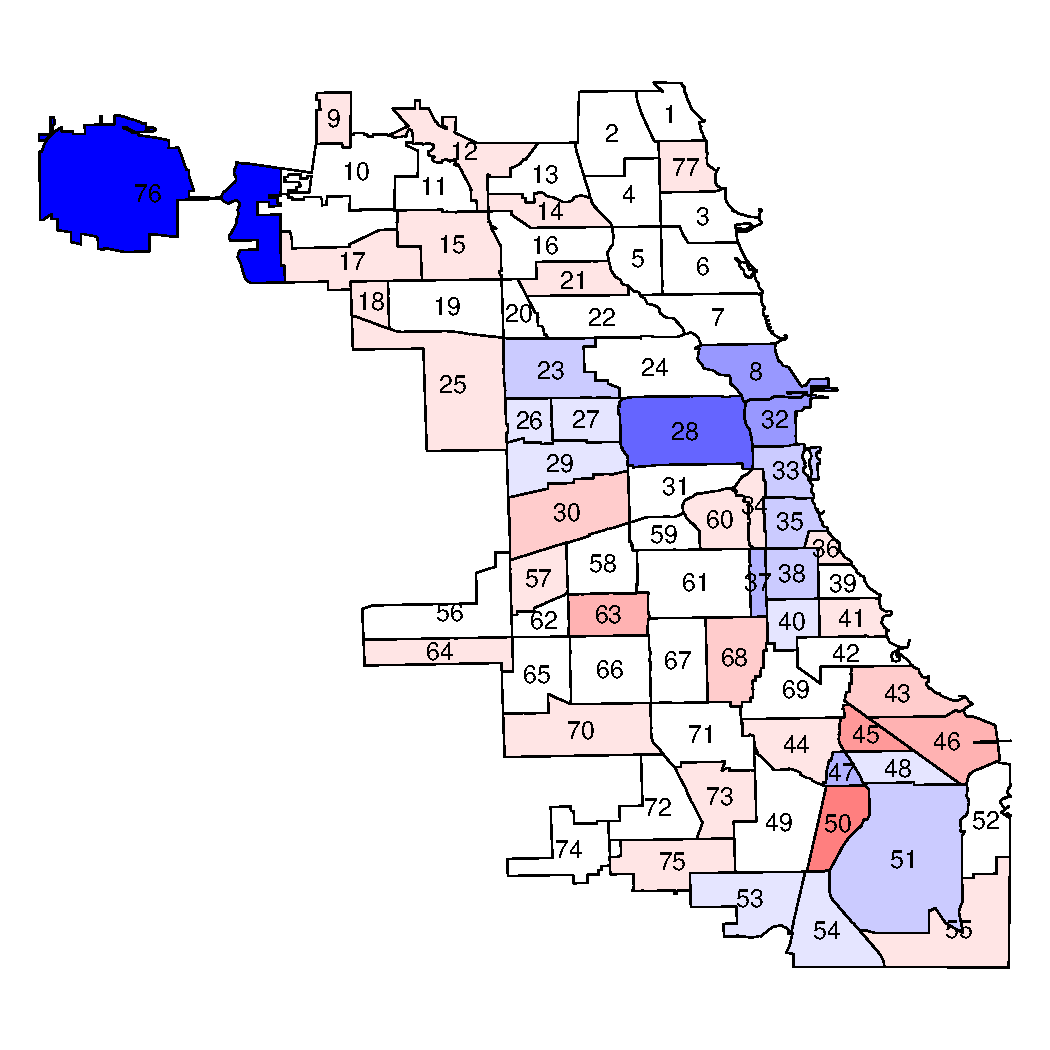
\includegraphics[width=0.45\textwidth]{fig/poi-improve.pdf}}
\subfigure[Taxi flow]{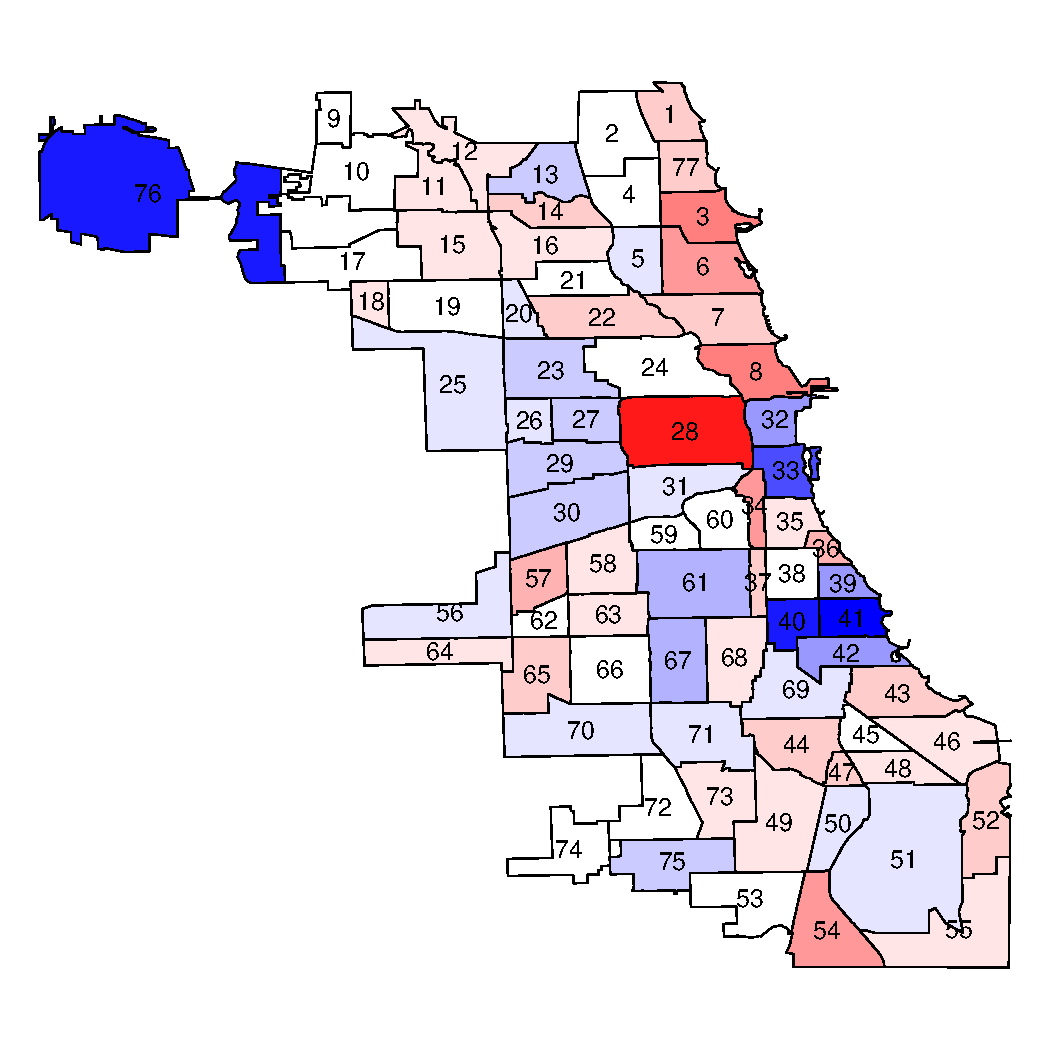
\includegraphics[width=0.45\textwidth]{fig/taxi-improve.pdf}}
\caption{Performance improvement per region by using POI or taxi flow features on 2014 crime. The difference of MAEs in estimating crime with/without POI feature is shown on the left, and the same measure of taxi flow is shown on the right. The color blue means the MAE is reduced by adding corresponding feature (i.e., better performance), while the red means the MAE is increased (i.e., worse performance). The color saturation indicates the value of difference.}
\label{fig:feat-area}
\end{figure}


It is interesting to find out that in the downtown area, i.e. community area \#8, \#32, \#28, and \#33, POI significantly improves the estimation accuracy. The reason is two fold. 1) The demographics information from census is mostly about the residing population in the focal area.  However, in the downtown area there are a lot of floating population groups conducting various social activities, and this is not reflected by the census demographics. The POI information, on the other hand, reflects the functionality of a region, and plays a complementary role of demographic information. 2) In the downtown area, there are much more POIs than any other places, which provides more complete information about the community profile.

As for the taxi flow feature, it helps the most in those suburb area, because the taxi flow reflects the social interaction in those areas. In the downtown, the taxi flow feature incurs a relatively large estimation error. The reason is that the taxi flow distribution in Chicago is extremely skewed. Roughly 61\% of the Chicago taxi trips have a destination in the downtown area, which may result in the model over-propagating crime estimates from all of Chicago into the downtown area.








\nop{
\medskip
\noindent \textbf{Evaluate on tract level}. \textred{The results are shown in Table~\ref{tb:evl-tract}. However, the improvement of adding new feature is not observed.}


\begin{table}[h]
\centering
\caption{Evaluation of crime in 2013 at tract level.}
\vspace{2mm}
\label{tb:evl-tract}
\begin{tabular}{|c|c|c|c|c|}
\hline
\multirow{2}{*}{Settings} & \multicolumn{2}{|c|}{LR} & \multicolumn{2}{|c|}{NB} \\ \cline{2-5}
	& MAE & MRE & MAE & MRE \\ \hline
D+S+P+T & 164.76 & 0.434 & 155.87 & 0.410 \\ \hline
D+S+T & 165.17 & 0.435 & 155.73 & 0.410 \\ \hline
D+S+P & 164.96 & 0.434 & 155.029 & 0.408 \\ \hline
D+S & 165.19 & 0.435 & 155.013 & 0.408 \\ \hline
D & 176.77 & 0.465 & 172.63 & 0.453 \\ \hline
\end{tabular}
\end{table}

}
